\documentclass{report}
\usepackage{fullpage}
\usepackage{tabu}
\usepackage{graphicx}
\usepackage{listings}
\usepackage{color}
\usepackage{hyperref}
 
\definecolor{codegreen}{rgb}{0,0.6,0}
\definecolor{codegray}{rgb}{0.5,0.5,0.5}
\definecolor{codepurple}{rgb}{0.58,0,0.82}
\definecolor{backcolour}{rgb}{0.95,0.95,0.92}
 
\lstdefinestyle{mystyle}{
    backgroundcolor=\color{backcolour},   
    commentstyle=\color{codegreen},
    keywordstyle=\color{magenta},
    numberstyle=\tiny\color{codegray},
    stringstyle=\color{codepurple},
    basicstyle=\footnotesize,
    breakatwhitespace=false,         
    breaklines=true,                 
    captionpos=b,                    
    keepspaces=true,                 
    numbers=left,                    
    numbersep=5pt,                  
    showspaces=false,                
    showstringspaces=false,
    showtabs=false,                  
    tabsize=2
}
 
\lstset{style=mystyle}
 


\renewcommand{\baselinestretch}{2}
\setlength{\parindent}{4em}
\setlength{\parskip}{1em}

\author{Author : Fahim Khan \\
		Mentor : Nilesh Khandelwal
}


\title{Market Regime Detection using Hidden Markov Model}
\begin{document}
\maketitle
\tableofcontents



\chapter{Objective}
There is always challenge for quantitative trader to find out the frequent behaviour of financial market due to change in government policy,negative news item,regulatory environment and other macroeconomics effects. Such periods are known as Market Regime.
These various regimes lead to adjustments of asset returns via shifts in their means, variances,
autocorrelation and covariances. This impacts the effectiveness of time series methods that rely on stationarity.
There is a clear need to effectively detect these regimes. This aids optimal deployment of quantitative trading strategies and tuning the parameters within them.\par

This project is an attempt to find out such market regime and accordingly adjust the strategy. The pricipal method used to detect market regime is known as Hidden Markov Model which is a statistical time series techinique.


\chapter{What is Hidden Markov Model?}
Before knowing about Hidden Markov Model, it important to understand Markov Model. The Markov Model is a stochastic state space model involves random transitions between states where the probability of the jump is only dependent upon the current state, rather than any of the previous states. The model is said to possess the Markov Property and is thus \textbf{memoryless}.

Markov Models can be categorised into four broad classes depending upon the autonomy
of the system and whether all or part of the information about the system can be observed at
each state.

 
 

\begin{tabu} to 0.8\textwidth { | X[l] | X[c] | X[r] | }
 \hline
  & Fully Observable & Partially Observable \\
 \hline
   Autonomous & Markov Chain  & Hidden Markov Model  \\
\hline
Controlled & Markov Decision Process  & Partially Observable Markov Decision Process \\
\hline
\end{tabu}

If model is both autonomous and fully observable. It cannot be modified by actions of an agent as in the controlled processes and all information is available from the model at any point in time.

If the model is fully autonomous but only partially observable then it is known as a Hidden Markov Model. In such a model there are underlying latent states and probability transitions between them but they are not directly observable. Instead these latent states influence the observations.

The HMM is more familiar in the speech recognition community and communication systems, but during the last years gained acceptance in finance as well as economics and management science.


\chapter{Implementation details}
\section{Programing Language}
The project has been implemented in Python version 2.7. Python being a open source language is most popular for data analysis as it has wide range of available packages for data analysis,machine learning and statistical analysis. It is very popular language and easy to use. 
\section{Packages}
The list of main packages used in this projects are as follows.

\begin{enumerate}
  \item Python (v2.7)
  \item Pandas (0.18.1)
  \item Numpy (1.13.1)
  \item Matplotlib (2.0.2)
  \item hmlearn (0.2.0)
\end{enumerate}

\section{Strategy}
As the main focus is on detection of market regime ,so I have used moving average strategy. As in case of HMM we can only have partially observable data, it become very important choose your observable data very carefully. For Moving average strategy I have choosen the daily returns as observable variable. We can also have daily std deviation ,daily volatility as observable variables.

In future work, I am going to add few more strategy with different observable variable.

\section{Data}

I have taken 120 days interaday data from Zerodha for the following script.
\begin{enumerate}
  	\item NIFTY50 Index
  	\item HDFCBANK
	\item ICICIBANK
	\item KOTAKBANK
	\item ONGC
	\item INFY
	\item RELIANCE
	\item HDFC
	\item LT
	\item IOC
	\item SBIN
	\item HINDUNILVR
	\item MARUTI
	\item ITC
	\item TCS
\end{enumerate}
It is always advisable to go for interaday data to get better result for detecting market regime using HMM.


\chapter{Backtesting Code}
All the backtesting code is written in \textbf{backtest.py} file. The file is divided into two class namely \textbf{FinancialData} and \textbf{BacktestBase}.

\section{FinancialData}
This class get all the data required for backtesting.
The class has following function.
\begin{itemize}
  \item \textbf{init :}
  It initialize with ticker name. Also profolio class object is initialized here.
  \item \textbf{get\_data :}
  All data reading happen in this function.
  Here we are loading the data in the pandas dataframe from csv file for the given ticker. You can load it from database 
  as well.
  \item \textbf{plot\_data :}
  This function plot the data on given column. By default it plot on close data.
\end{itemize}


\section{BacktestBase}
This class inherit all the property of FinacialData. Which means I can access the get\_data and plot function from this class as well. This class has follwing function.

\begin{itemize}
  \item \textbf{init :}
  It initialize with initial amount invested, amount after all backtesting,no of trades ,units ,position and transaction cost based on broker. I am calculating brokerage charge as per zerodha brokerage. So I am not using ftc and ptc.
  \item \textbf{get\_trade\_price :}
  This function gives the current trade price based on number of units.Also it add the transaction cost to it.
  \item \textbf{get\_date\_price :}
  This functon give the price of security at current data index level.
  \item \textbf{get\_txn\_cost :}
  Based on the amount invested it calculates the transaction cost.This function may change based on different broker.
  \item \textbf{get\_trade\_units :}
  This function gives the number of units you can buy based on the available amount.
  \item \textbf{place\_buy\_order :}
  This function place the buy order and accordingly modify the trade details,units and available amount.
  \item \textbf{place\_sell\_order :}
  This function place the sell order and accordingly modify the trade details,units and available amount.
  \item \textbf{trade\_stats :}
  This function give the trade status once the backtesting is completed. Here I am calculating,initial amount invested, final balance, performance,number of trades and sharpe ratio.
  You can calculate your own stat here.

\end{itemize}

\section{Portfolio}
This class is written in \textbf{portfolio.py}. It actuallly being called from \textbf{trad\_stat} function for each and every symbol. This class is reponsible for maintaing the portfolio details of every symbol on which we want to run tht backtesting strategy. Her we can find out which symbol is performing better for our backtesting strategy and we can focus on those symbol in live trading.

Portfolio class has following methods.

\begin{itemize}
  \item \textbf{init :}
  It initialize portfolio details which hold column name for our portfolio stats.
  \item \textbf{add\_portfolio\_details :}
  This function add the portfolio details for every individual ticker.
  \item \textbf{show\_portfolio\_details :}
  This function actually store the portfolio details object in the pickel file and save on disk which can be load at anytime for comaparision , presentation etc.
  

\end{itemize}



\chapter{Training model for HMM}
It is important to split the data into training and test data into proper ratio. As I have only 120 days interaday data it was difficult for me to have 70:30 ratio so I have decided to split it into 50:50 ratio. Please note that more the amount of data better would be the result. If you have large data the I would suggest you to go with 70:30 split which can be optimized.

The file used for training model is \textbf{hmm\_regime\_training\_model.py}.
This code actually split the data into training and test data in 50:50 ratio. To create the model \textbf{hmmlearn} package of python has been used. Please note that while creating the model it is important to choose the observable variable very carefully as on this variable model is going to be fit.Here in moving average startegy the observable variable is \textbf{daily returns}. We can also use \textbf{standard deviation, volatility, forward volatilty(for options) etc.}

Once the model is created, it is dumped to a file using same \textbf{pickle} module of python. It creates file for each and every symbol and store it into \textbf{Model} directory. 

\newpage

The code snippet for training HMM model is as follow.

\begin{lstlisting}[language=Python]
import warnings
import pandas as pd
import datetime
import numpy as np
import pickle
from hmmlearn.hmm import GaussianHMM

data_location = "../Data/IntraDay/"
train_test_split_ratio  = 0.5


# Hides deprecation warnings for sklearn
warnings.filterwarnings("ignore")
tickerList = ["HDFCBANK","ICICIBANK","KOTAKBANK","ONGC","INFY","RELIANCE","HDFC","LT","IOC","SBIN","HINDUNILVR","MARUTI","ITC","TCS"]

for ticker in tickerList:
	model_path = "../Models/hmm_model_"+ticker+".pkl"
	data = pd.read_csv(data_location+ticker+"-EQ.csv",index_col='Date',names=['Date','Open','High','Low','Close','Volume'],skiprows=1) 
	data["Returns"] = data["Close"].pct_change() 
	data.dropna(inplace=True)
	#Reverse data to get proper ascending order
	data =  data.iloc[::-1]   
	
	##Split data into training and test data
	training_data_len = int(len(data)*train_test_split_ratio) ##TO get training data
	end_date = data.index[training_data_len]
	start_date = data.index[training_data_len+1]
	training_df = data[:end_date]
	test_df =  data[start_date:]
	# print training_df.tail()
	# print test_df.head()
	
	##Observable valriable on which hmm model will fits
	returns = np.column_stack([training_df["Returns"]])
	
	# Create the Gaussian Hidden markov Model and fit it
	# to the returns cloumns fo training data, outputting a score
	hmm_model = GaussianHMM(n_components=2, covariance_type="full", n_iter=1000).fit(returns)
	
	#Dump model in a file to use it later on
	pickle.dump(hmm_model, open(model_path, "wb"))


\end{lstlisting}



\chapter{Strategy code without using HMM}
The file used to create moving average strategy is \textbf{moving\_average.py}.
If we run this file , it will run the moving average strategy on all the listed security given in the list.
Also, you can declare inital amount to be invested. The portfolio object will give you the final status and also save it on disk for future use.

\begin{lstlisting}[language=Python]
tickerList = ["HDFCBANK","ICICIBANK","KOTAKBANK","ONGC","INFY","RELIANCE","HDFC","LT","IOC","SBIN","HINDUNILVR",
	"MARUTI","ITC","TCS"]

	initial_investement_amount = 10000

	for ticker in tickerList:
		sma = MovingAverageStrategy(ticker,initial_investement_amount)
		sma.run(50,250)

	portOBJ = Portfolio()
	portOBJ.show_portfolio_details("port_without_hmm.pkl")
\end{lstlisting}

\section{MovingAverageStrategy}
This class implement the moving average strategy. The class inherits the BacktestBase which inherits FinancialData class. So, basically it has access to data as well as backtesting class. 

It only has \textbf{run} method which is called to execute strategy on a given symbol and data. It copy the data into another data frame and do not touch origianl data frame.It split the data into 50:50 ratio same as we did it in training mode section. Please note that, here we only have to run the strategy on testing data only even though we are using moving average without HMM. Because if we run the strategy on whole data then it would be useless to compare the result between startegy with HMM and strategy without HMM as strategy with HMM will run on test data only as training data will be used for training model.

The complete code for moving average is as follow.

\begin{lstlisting}[language=Python]
import pandas as pd
import numpy as np

from backtest import BacktestBase
from portfolio import Portfolio

train_test_split_ratio  = 0.5


class MovingAverageStrategy(BacktestBase):
	def run(self,SMA1,SMA2):
		msg = 'Running SMA strategy for %s |SMA1 =%d |SMA2 = %d |ftc = %f|ptc = %f'
		msg = msg%(self.ticker,SMA1,SMA2,self.ftc,self.ptc)
		self.position = 0
		self.amount = self.initial_amount
		self.trades = 0


		#Data Preparation
		self.data_run = self.data.copy()
		self.data_run['SMA1'] = self.data_run['Close'].rolling(SMA1).mean()
		self.data_run['SMA2'] = self.data_run['Close'].rolling(SMA2).mean()
		self.data_run["Returns"] = self.data_run["Close"].pct_change() 
		self.data_run.dropna(inplace=True)


		##Split data into training and test data
		training_data_len = int(len(self.data_run)*train_test_split_ratio) ##TO get training data
		end_date = self.data_run.index[training_data_len]
		start_date = self.data_run.index[training_data_len+1]
		training_df = self.data_run[:end_date]
		test_df =  self.data_run[start_date:]

		#Running for test data only
		self.data_run = test_df
		

		# print self.data_run.head()

		########Signals
		Signals = pd.DataFrame(index=self.data_run.index)
		Signals["PnL"] = 0
		Signals["Trade"] = 0
		Signals["Units"] = 0
				
		for bar in range(0,len(self.data_run)):
			if self.position == 0:
				if self.data_run['SMA1'].ix[bar] > self.data_run['SMA2'].ix[bar]:
					self.place_buy_order(bar,amount=self.amount) 
					self.position = 1 #Take Position
					Signals["Trade"].ix[bar] = 1
					Signals["Units"].ix[bar] = int(self.units)
				else:
					Signals["Trade"].ix[bar] = 0
					
			elif self.position == 1:
				if self.data_run['SMA1'].ix[bar] < self.data_run['SMA2'].ix[bar]:
					Signals["Units"].ix[bar] = int(self.units)
					self.place_sell_order(bar,units=self.units)
					self.position = 0   #Market nuetral
					Signals["Trade"].ix[bar] = -1
				else:
					Signals["Trade"].ix[bar] = 0
				
		
		##Squaring off if holds any stock without checking any condition
		if self.position == 1:
			Signals["Units"].ix[bar] = int(self.units)
			self.place_sell_order(bar,units=self.units)
			self.position = 0   #Market nuetral
			Signals["Trade"].ix[bar] = -1


		##Concatenating both dataframe
		frames = [self.data_run,Signals]
		self.final_dataframe = pd.concat(frames,axis=1, join_axes=[self.data_run.index])
		
		
		##PnL
		price=0.
		for bar in range(0,len(self.final_dataframe)):
			if self.final_dataframe['Trade'][bar] == 1:
				price = self.get_trade_price(bar,self.final_dataframe['Units'][bar])
			elif self.final_dataframe['Trade'][bar] == -1:
				self.final_dataframe['PnL'].ix[bar] = self.get_trade_price(bar,self.final_dataframe['Units'][bar]) - price
			
		self.trade_stats(bar,self.final_dataframe)

if __name__ == "__main__":
	tickerList = ["HDFCBANK","ICICIBANK","KOTAKBANK","ONGC","INFY","RELIANCE","HDFC","LT","IOC","SBIN","HINDUNILVR",
	"MARUTI","ITC","TCS"]

	initial_investement_amount = 10000

	for ticker in tickerList:
		sma = MovingAverageStrategy(ticker,initial_investement_amount)
		sma.run(50,250)

	portOBJ = Portfolio()
	portOBJ.show_portfolio_details("port_without_hmm.pkl")

\end{lstlisting} 


\chapter{Strategy code with using HMM}
The file used to create moving average strategy with using HMM is \textbf{moving\_average\_using\_hmm.py}.
If we run this file , it will run strategy on all the listed security given in the list.
Also, you can declare inital amount to be invested. The portfolio object will give you the final status and also save it on disk for future use.

It first load the model which we have trained in previouse chapter. It keeps adding daily returns to a list from test data.And whenever the strategy go for trade it actually first check if any regime is detected by feeding daily returns(Observable data) to HMM model. And if model got any regime the strategy would not trade and also it will sqaure off any holdings as well.

\newpage

The function to detect regime is as follow.

\begin{lstlisting}[language=Python]
def regime_detection(self,daily_returns):
		#Converting daily return list to numpy array
		daily_returns = np.column_stack([np.array(daily_returns)])
		hidden_state = self.hmm_model.predict(daily_returns)[-1]
		return hidden_state

\end{lstlisting}

If the function returns 1 it will not trade and squareoff if it has any holdings. Otherwise it will work as normal strategy.

The complete code snippet for moving average strategy with using HMM is as follow.

\begin{lstlisting}[language=Python]

import pandas as pd
import numpy as np
import pickle

from backtest import BacktestBase
from portfolio import Portfolio


train_test_split_ratio  = 0.5

class MovingAverageStrategy(BacktestBase):
	def run(self,SMA1,SMA2,model_path):
		daily_returns = []
		msg = 'Running SMA strategy for %s |SMA1 =%d |SMA2 = %d |ftc = %f|ptc = %f'
		msg = msg%(self.ticker,SMA1,SMA2,self.ftc,self.ptc)
		self.position = 0
		self.amount = self.initial_amount
		self.trades = 0

		self.hmm_model = pickle.load(open(model_path, "rb"))


		#Data Preparation
		self.data_run = self.data.copy()
		self.data_run['SMA1'] = self.data_run['Close'].rolling(SMA1).mean()
		self.data_run['SMA2'] = self.data_run['Close'].rolling(SMA2).mean()
		self.data_run["Returns"] = self.data_run["Close"].pct_change() 
		self.data_run.dropna(inplace=True)


		##Split data into training and test data
		training_data_len = int(len(self.data_run)*train_test_split_ratio) ##TO get training data
		end_date = self.data_run.index[training_data_len]
		start_date = self.data_run.index[training_data_len+1]
		training_df = self.data_run[:end_date]
		test_df =  self.data_run[start_date:]

		#Running for test data only
		self.data_run = test_df
		

		# print self.data_run.head()

		########Signals
		Signals = pd.DataFrame(index=self.data_run.index)
		Signals["PnL"] = 0
		Signals["Trade"] = 0
		Signals["Units"] = 0
				
		for bar in range(0,len(self.data_run)):
			##Storing observable varibale.In our case it is daily returns.
			daily_returns.append(self.data_run['Returns'].ix[bar])

			regime = self.regime_detection(daily_returns)

			if self.position == 0:
				if regime == 1:
					pass
				else:
					if self.data_run['SMA1'].ix[bar] > self.data_run['SMA2'].ix[bar]:
						self.place_buy_order(bar,amount=self.amount) 
						self.position = 1 #Take Position
						Signals["Trade"].ix[bar] = 1
						Signals["Units"].ix[bar] = int(self.units)
					else:
						Signals["Trade"].ix[bar] = 0
					
			elif self.position == 1:
				if regime == 1:
					print "Sell Without condition"
					Signals["Units"].ix[bar] = int(self.units)
					self.place_sell_order(bar,units=self.units)
					self.position = 0   #Market nuetral
					Signals["Trade"].ix[bar] = -1
				else:
					if self.data_run['SMA1'].ix[bar] < self.data_run['SMA2'].ix[bar]:
						Signals["Units"].ix[bar] = int(self.units)
						self.place_sell_order(bar,units=self.units)
						self.position = 0   #Market nuetral
						Signals["Trade"].ix[bar] = -1
					else:
						Signals["Trade"].ix[bar] = 0

			
				
		
		##Squaring off if holds any stock without checking any condition
		if self.position == 1:
			Signals["Units"].ix[bar] = int(self.units)
			self.place_sell_order(bar,units=self.units)
			self.position = 0   #Market nuetral
			Signals["Trade"].ix[bar] = -1


		##Concatenating both dataframe
		frames = [self.data_run,Signals]
		self.final_dataframe = pd.concat(frames,axis=1, join_axes=[self.data_run.index])
		
		
		##PnL
		price=0.
				
		for bar in range(0,len(self.final_dataframe)):
			if self.final_dataframe['Trade'][bar] == 1:
				price = self.get_trade_price(bar,self.final_dataframe['Units'][bar])
			elif self.final_dataframe['Trade'][bar] == -1:
				self.final_dataframe['PnL'].ix[bar] = self.get_trade_price(bar,self.final_dataframe['Units'][bar]) - price 
	

		self.trade_stats(bar,self.final_dataframe)

	def regime_detection(self,daily_returns):
		#Converting daily return list to numpy array
		daily_returns = np.column_stack([np.array(daily_returns)])
		hidden_state = self.hmm_model.predict(daily_returns)[-1]
		return hidden_state


if __name__ == "__main__":
	tickerList = ["HDFCBANK","ICICIBANK","KOTAKBANK","ONGC","INFY","RELIANCE","HDFC","LT","IOC","SBIN","HINDUNILVR",
	"MARUTI","ITC","TCS"]

	initial_investement_amount = 10000

	for ticker in tickerList:
		model_path = "../Models/hmm_model_"+ticker+".pkl"
		sma = MovingAverageStrategy(ticker,initial_investement_amount)
		sma.run(50,250,model_path)


	portOBJ = Portfolio()
	portOBJ.show_portfolio_details("port_with_hmm.pkl")


\end{lstlisting}


\chapter{Findings}
The portfolio details has been saved as pickle object which can be loaded and see the result. To read the result please look at file \textbf{Read\_Portfolio.py}

This file just load the result file and print it in human readable format. The code snippet is as follows.
\begin{lstlisting}[language=Python]
import pandas as pd

port_without_hmm = pd.read_pickle("port_without.pkl")
port_with_hmm = pd.read_pickle("port_with.pkl")

print "#######Portfolio Wihtout using HMM##########"
print port_without_hmm

print "###############Portfolio with using HMM############"
print port_with_hmm

\end{lstlisting}

\newpage
The result for moving average strategy without using HMM shown in figure \ref{fig:no_hmm}.

\begin{figure}[h!]
  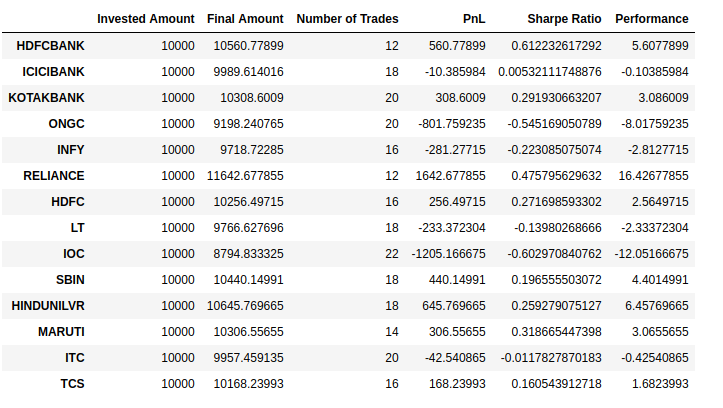
\includegraphics[width=15cm, height=8cm]{Result_Without_HMM.png}
  \caption{Result without HMM.}
  \label{fig:no_hmm}
\end{figure}

\newpage
The result for moving average strategy with using HMM shown in figure \ref{fig:hmm}.

\begin{figure}[h!]
  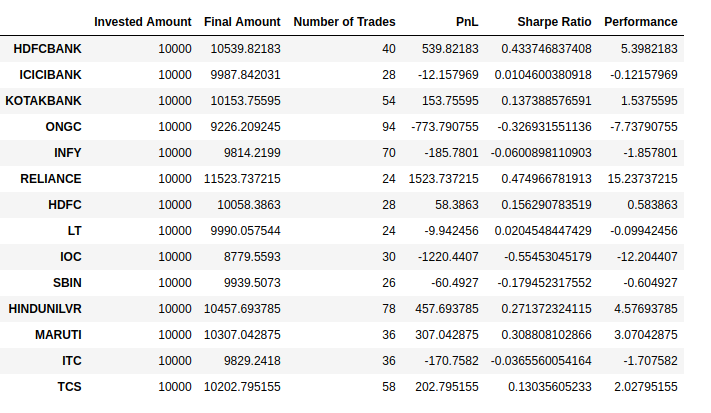
\includegraphics[width=15cm, height=8cm]{Result_With_HMM.png}
  \caption{Result with HMM.}
  \label{fig:hmm}
\end{figure}


We can see that there are bunch of security which has performed well without using HMM such as \textbf{KOTAKBANK},\textbf{HINDUNILVR} and \textbf{RELIANCE}. But our profit is not in negative. It  is just that we earned little less profit.

Now if we comppare the result for security \textbf{ONGC},\textbf{INFY},\textbf{LT},\textbf{SBIN}. We can see that loss has been reduced sharply for strategy using HMM. In fact one of the security \textbf{TCS} which was in loss is giving us profit.

If you see the overall picture, we can conclude that startegy with HMM may give you little less profit but it will save you from the major losses during regime change. We can use HMM with any startegy for risk management purpose.

The result we are comparing is just for 120 days interaday data. We can actually use the large data set to see how HMM perform with your startegy for risk management.


\chapter{Future Work}
We can do lot of thing to improve the HMM model. I have listed few of them which I will try to do it in future.

\begin{itemize}
\item Running different startegy with HMM such as mean reversion,pair trading.
\item Changing observable varibale to std deviation,volatilty etc
\item Optimizing training and test data split by using large data set. 
\end{itemize}


\chapter{Reference}

\begin{itemize}
\item \url{https://en.wikipedia.org/wiki/Hidden_Markov_model}
\item \url{https://www.quantstart.com/}
\item \url{https://www.python.org/}
\item \url{http://hmmlearn.readthedocs.io/en/latest/tutorial.html}
\end{itemize}




\end{document}
